\chapter{Data Collection}

This chapter will discuss the data collection task, participants and responses.

\section{Picture Description Task}
\label{sec:pdt}

%\subsection{PDT Stimuli}

The PDT is built around 30 images. Each image is a simple, cartoon-like vector graphic. These images were either purchased online or found in publicly available graphics libraries. In order to constrain response contents to the main focus of each image, the images were modified to remove any non-essential detail or background. Vector graphics are ideal for this task, because they tend to have an illustrational style with very little detail, as compared to photographs or drawings. Moreover, most consist of layers of graphic objects, and these objects can be easily moved, resized, deleted, combined or otherwise modified to compose the desired stimulus. Example images are presented in Table~\ref{tab:example-pdt-items} and the full set is contained in Appendix XYZ \lk{XYZ=?}. To factor out the influence of previous linguistic context, images are intentionally devoid of any text or symbols. The only exceptions to this are two images with music notes, one with a legible analog clock, one with numerals in an arithmetic problem, and one with a question mark.

Each image was chosen for its depiction of an ongoing or imminent action, performed by a person or an animal. The images are divided evenly into actions that are canonically intransitive, transitive and ditransitive in English.

Each PDT image is used in two different contexts: \textbf{targeted} and \textbf{untargeted}. An \textbf{item} consists of an image and a prompt question. For \textbf{targeted} items, questions take the form of \textit{What is $<$subject$>$ doing?}, with the subject provided (e.g., \textit{the boy}, \textit{the bird}). For all \textbf{untargeted} items, the question is \textit{What is happening?} Thus, there are a total of 60 different items used in this study. Collecting these targeted and untargeted responses allows for the examination of response variation with and without a subject constraint, thereby informing approaches to task design and automatic content assessment \citep{foster2009native, cho2013investigating}. 

Multiple versions of the PDT were necessary to collect roughly equal numbers of targeted and untargeted \textbf{responses} for each image. These versions vary in which images are presented as targeted items and which images are presented as untargeted items. Additionally, NSs were asked to provide two non-identical responses to each item, but NSs were asked to provide only one response per item, so different PDT versions were used for these groups. The PDTs were hosted online via Survey Monkey, and all participants submitted their responses through this platform. Survey Monkey restricts the number of questions included in surveys used for purchasing crowdsourced responses, so the PDTs were split accordingly for this group.

In each (full-length) PDT, targeted items are presented in the first half, and untargeted items are presented in the second half. This targeted-untargeted ordering is intended to avoid the possibility that in an untargeted-targeted task, respondents might notice that the question for each untargeted item is the same in the first half and finish the task hastily without noticing that later targeted items specify the subject. Each half is introduced with instructions, including an example item with sample responses. The instructions ask participants to focus on the main event depicted in the image and for each response to be one complete sentence. The PDT was presented as an online survey, and all participants typed their responses. Participants were instructed not to use any reference materials, but browser-based spell checking was not disabled, and participants are assumed to have used it as necessary.

A complete paper-based version of the PDT is included in Appendix XYZ \lk{XYZ=?} and the full set of PDT versions is available for download with the SAILS Corpus.\footnote{https://github.com/sailscorpus/sails} The main task instructions are presented in (\ref{exe:pdt-instructions-a}). Additional instructions provided to NSs are presented in (\ref{exe:pdt-instructions-b}).

\begin{exe}
  \ex\label{exe:pdt-instructions-a}In this task, you will view a set of images. For each image, please write \textbf{one sentence} to answer the question provided with the image. It is important to write a \textbf{complete sentence}, not a word or phrase.
\end{exe}

\begin{exe}
  \ex\label{exe:pdt-instructions-b}Then, you will be asked to write a second, \textit{different} answer, which is also a complete sentence. This might involve rewording or reorganizing your first sentence. It does not need to be \textit{completely} different; some words may be the same. If you cannot think of another way to answer the question, you may leave the second answer space empty, but any second responses you provide will be greatly appreciated.
\end{exe}

%% LK NTS:
%%intransitive is I30 (woman is running)
%%transitive is I29 (woman is hugging dog)
%%ditransitive is I28 (man is giving directions)
\begin{table}[htb!]
%\begin{table}[t!] This line is giving me trouble when I go to typeset
\begin{center}
\begin{tabular}{|c|c|c|}
\hline
{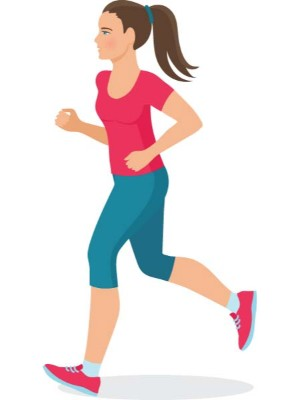
\includegraphics[width=0.29\columnwidth]{figures/I30.jpg}} & {
\includegraphics[width=0.3\columnwidth]{figures/I29.jpg}} & {
\includegraphics[width=0.3\columnwidth]{figures/I28.jpg}} \\
\hline
What is the woman doing? & What is the woman doing? & What is the man doing? \\
\hline
\end{tabular}
\caption{\label{tab:example-pdt-items} PDT example images with their targeted questions. In the untargeted form, the question for each is \textit{What is happening?} From left to right, the examples represent one intransitive, transitive and ditransitive item.}
\end{center}
\end{table}


%\subsection{Data Collection}
\section{Participants}
\label{sec:participants}

This study involved a total of 499 PDT participants. Of these, 141 were NNSs, recruited from intermediate and advanced writing courses for English as a Second Language students attending Indiana University. These participants performed the task in a computer lab with the researchers present. They were native speakers of Mandarin Chinese (125), Korean (4), Burmese (3), Hindi (2), and one native speaker each of Arabic, Indonesian Bahasa, German, Gujarati, Spanish, Thai and Vietnamese. Because nearly 90\% of these recruits were native speakers of Chinese, care should be taken when drawing conclusions from the corpus; patterns observed among the NNSs here might not apply broadly to all NNSs. 

Of the 358 NS participants, 29 were personally known and recruited by the researcher. Throughout this work, these participants will be referred to as the \textbf{Familiar Native Speakers (FNSs)}. Responses from the remaining 329 NSs were purchased via Survey Monkey, an online survey platform. These participants will be referred to as the \textbf{Crowdsourced Native Speakers (CNSs)} where participants earn credits they can redeem for gift cards and prizes. Due to length restrictions for purchased surveys, these NSs each completed only half of the task, so their data is equivalent to 164.5 full participants.

All participants completed a background questionnaire at the beginning of the PDT. This included questions about first and second languages, gender, age, national origin, amount of English language instruction and length of residency in English-speaking locations. This questionnaire is included as part of the PDT in Appendix XYX. \lk{XYZ}

In previous similar work \citep{king:dickinson:13},
%\citep{king:dickinson:13,king:dickinson:16},
NSs were found to produce less variation than NNSs. Many NSs provided identical responses or responses that hew very closely to the most canonical way of expressing the main action. A major motivation for collecting the corpus here is to be able to assess NNS response content by comparing it against the NS responses. For this reason, NSs were asked to provide two non-identical responses, in the hopes that this would result in more examples of native-like responses for the NNS responses to compare against.

\section{Responses}
\label{sec:responses}

\begin{table}[htb!]
\begin{center}
\begin{tabular}{|l||r|r||r|}
\hline
& \multicolumn{3}{|c|}{Response Counts} \\
\hline
 Group & First & Second & Total \\
\hline
\hline
NNS & 4290 & 0 & 4290 \\
\hline
\hline
NS (all) & 4634 & 4609 & 9243 \\ %%LK: Yes, 0.949 is correct in both cases here
\hline
\multicolumn{1}{|r||}{FNS} & 642 & 641 & 1283 \\ 
\hline
\multicolumn{1}{|r||}{CNS} & 3992 & 3968 & 7960 \\
\hline
\hline
Total & 8924 & 4609 & 13,533 \\
\hline
\end{tabular}
\caption{\label{tab:response-counts} First and second response counts for the corpus participant groups. Familiar (FNS) and crowdsourced (CNS) are subgroups of NS. NNS participants are not asked to provide a second response.}
\end{center}
\end{table}

To examine the degree of variation among the NSs and NNSs  in the current study, type-to-token ratios (TTR) were calculated on the response level for the entire set of items, shown in Table~\ref{tab:ttr}. For this calculation, final punctuation was ignored, and all responses were converted to lowercase. To illustrate, the three response \textit{tokens} in (\ref{exe:ttr-1}), (\ref{exe:ttr-2}) and (\ref{exe:ttr-3}) would constitute a single response \textit{type}.

\begin{exe}[h!]
  \ex\label{exe:ttr-1}The woman is holding a dog
\end{exe}
\begin{exe}[h!]
  \ex\label{exe:ttr-2}the woman is holding a dog!
\end{exe}
\begin{exe}[h!]
  \ex\label{exe:ttr-3}The Woman is holding a Dog.
\end{exe}

For each data point in the table, the corpus contains roughly 150 NS responses and 70 NNS responses. To control for this imbalance and its effect on the likelihood of seeing new responses, the TTR was calculated for each item based on a random sample of 50 responses.  This was repeated 10 times and then averaged to produce a final TTR each item. Then, for intransitives, transitives and ditransitives, the TTR was calculated as the average TTR of the 10 items in each set. The scores in in Table~\ref{tab:ttr} show that in all cases, the NS set shows a greater degree of response variation, meaning that asking for two responses appears to be an effective way of collecting a broader range of NS responses.

\begin{table}[hb!]
\begin{center}
\begin{tabular}{|l||l|l||l|l|}
\hline
 & \multicolumn{2}{|c||}{Targeted} & \multicolumn{2}{|c|}{Untargeted} \\
\hline
 Set & NS & NNS & NS & NNS \\
\hline
\hline
Intrans & 0.628 & 0.381 & 0.782 & 0.492 \\
\hline
Trans & 0.752 & 0.655 & 0.859 & 0.779 \\ %%LK: Yes, 0.949 is correct in both cases here
\hline
Ditrans & 0.835 & 0.817 & 0.942 & 0.936 \\ 
\hline
\end{tabular}
\caption{\label{tab:ttr} NS and NNS type-to-token ratios (TTR) for complete responses (not words), for the full corpus.}
\end{center}
\end{table}

\textbf{*Let's separate 1st and 2nd responses and calculate the TTRs this way also*}\lk{1st vs 2nd responses}

The ratios show the direct relationship between the complexity of the event portrayed (represented here as intransitive, transitive and ditransitive) and the degree of variation elicited. In all cases, TTR increases with this complexity. Interestingly, this trend seems more pronounced in the NNS responses; in the targeted NNS responses, the TTRs for intransitive and ditransitive items are 0.381 and 0.817, respectively, compared to 0.628 and 0.835 for NS responses. \textbf{*Might this be explained by the inclusion of NNS 2nd responses? Let's investigate*}\lk{1st vs 2nd?} The ratios also show that in all cases, as expected, variation is greater for untargeted items than it is for targeted items. In other words, asking about a particular subject in the prompt question does constrain the variety of responses.

